\subsection{Decision Range (DR) and Abort/Skate/Banzai}

\subsubsection*{Simple Definitions}

\begin{itemize}
  \item Abort: Egress from an engagement without intent to recommit.

  \item Skate: Egress from an engagement with possible/likely option to
    recommit.

  \item Decision Range: NLT range from target allowing time to perform a Notch
    and assess before reaching MAR

  \item Banzai: Head into the merge (press).

  \item F-Pole: The distance from launcher to target if the shot was taken now.

  \item MAR: Minimum Abort Range; the closest Range at which you can safely
    turn from the fight and run from a specific enemy missile.

\end{itemize}

\subsubsection*{General}

Once in the Crank, the flight has to monitor several items:

\begin{itemize}
  \item RWR - Enemy Spikes (Plane and Missile)
  \item Defending via chaff
  \item Gimbals and missile support
  \item Pitbull and Timeout
  \item Relative altitude differences (avoiding being notched)
  \item Enemy defending (opportunities to Banzai)
  \item Range, especially Minimum Abort Range
\end{itemize}

Culminating in a decision to Banzai, Skate or Abort.

This phase is quite complex and of the highest workload.

\sidebyside{0.5}{%
  So far the flight has given good initial launch energy to the missile shot,
  then increased the Bandit's F-pole to increase the travel distance of a
  return shot. At the point where there are missiles in the air and possibly
  returned shots, the flight leader has to concern themselves with what to do
  next.
}{
  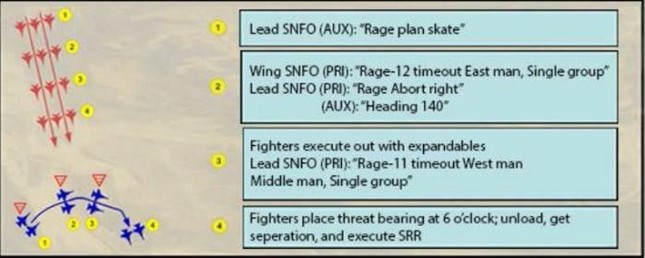
\includegraphics[width=\textwidth,align=t]{bvr/decision}
}

The safest goal for a long shot is to Skate out and exit the fight with an open
mind to recommit, once the missile is properly under its own guidance.
\textbf{The Tomcat should never choose to merge whilst other options
exist to succeed in the mission}. The flight can still monitor the shot using
the "Time To Impact" (TTI) timer displayed to the right of the target's TWS
track symbol.

Once the TTI starts to flash, the Missile Active command has been sent and the
Phoenix and can be considered 'Pitbull'. Depending on the TGTS target size
switch setting, the Missile Active command is sent at a calculated range from
target of 13nm (LARGE), 10nm (NORM) or 6nm (SMALL) - this usually translates to
remaining TTIs of around 20, 15 or 8 seconds from calculated impact.

Upon Pitbull the Pilot should put the enemy on the 3-9 line and notch. At this
point the crew are looking for Spikes/Nails, releasing chaff, observing the
relative aspect and altitude of the Bandit and its range for determining the
Minimum Abort Range (MAR). Knowing the Bandit's MAR is a matter of briefing and
experience.

Should the Bandit drop their spike and appear defensive in aspect or altitude
change, the choice to Press or "Banzai" could be made

\boxed{%
  Note: Most of this is advanced and kept for CT and
  \href{https://cloud.132virtualwing.org/s/DdLFQX4LLTExij2}{132\nd Air to Air
  TTP}. For now, all that is required to know is that there are three choices
  and three possible calls on Pri; to "Banzai", "Skate" or to "Abort".
}

\subsubsection*{Example}


\textbf{FL RIO (Pri):} "1, Pitbull!"\\
\textbf{WM RIO (Pri):} "2, Pitbull!"\\
\textbf{FL RIO (Pri):} "1, Timeout and Naked, Spectre, Banzai!"\\

\textbf{Or}

\textbf{FL RIO (Pri):} "1, Pitbull!"\\
\textbf{FL RIO (Pri):} "1, Spiked"\\
\textbf{FL RIO (Pri):} "Spectre 1, Abort 180"\\

\boxed{%
  Both RIO's will call out Spikes on RWR and transitions to Naked or any change
  thereof. They will also monitor their own shot and report both Pitbull and
  Timeout if possible. At Pitbull they stop keeping the target track inside
  gimbal limits and put any threat on the 3-9 before making a decision on
  whether to Abort or Banzai.
}
